\section{Quality Management}
This chapter documents the necessary information required to effectively manage project quality from project planning to delivery. It defines a project’s quality roles, responsibilities, tools, procedures and authorities.
\label{sec:quality}
\lhead{\thesection \space Quality Management}
\subsection{Plan Quality Management}
To ensure a sufficient quality level, every member of the team is involved in the quality process sharing responsibilities. The product owner is involved by providing the test framework.
\begin{table}[H]
\centering
\begin{tabular}{|c|c|l|}
\hline
\cellcolor{gray}Name & 
\cellcolor{gray}Role &
\cellcolor{gray}Responsibilities \\\hline
Guido Bruzniak & Product owner &
- Quality mentoring and coaching.\\\hline
Lucas Gehlen&Team member&- Taking part in code reviews.\\
Marco Kull&&- Writing code tests.\\
Patrick Richter&&- Quality audits.\\
Sebastian Wilczek&&- Doing manual GUI testing.\\\hline
\end{tabular}
\caption{Quality Roles \& Responsibilities}
\end{table}
\subsection{Perform Quality Assurance}
How the quality test will be performed depends on the type of the module being tested.\\
Design fragments and frontend modules are reviewed and, in case of front end modules, manually tested. They are then presented and discussed by the whole team and the product owner at the weekly meetings.\\
Backend modules are also reviewed by one team member, but the review includes writing firebase unit tests for it.\\

\subsection{Control Quality}
\begin{table}[!ht]
  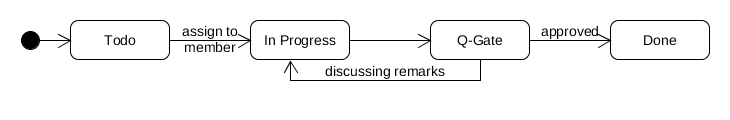
\includegraphics[width=\linewidth]{content/diagram/quality/state-quality.png}
  \caption{Quality process}
\end{table}
To ensure complete quality testing on the software every completed part will be assigned to a quality testing state. A team member that has not been part of the creation of the relevant piece then performs the quality testing.